\subsection{Background Subtraction}
\label{subsection:training}

Background subtraction is the process of determining which pixels belong to the background and which are foreground objects. The Gaussian Mixture Model method of clustering (\ref{subsection:mog}) was used to group pixels into foreground and background classes, where the foreground pixel class contains vehicle objects. The background subtractor takes video of the traffic scenario as input and returns a binary output image where all foreground pixels are white and background pixels are black, known as a foreground mask. 

This component of the algorithm was the most computationally expensive but because image processing was required to occur in real-time it was imperative that a fast implementation was used. Fortunately the OpenCV's BackgroundSubtractorMOG2 function \cite{opencv_mog2} is both fast and effective making it a suitable choice for a low power microcontroller. OpenCV's Mixture of Gaussians implementation is based on the the research by Zoran Zivkovic and Ferdinand van der Heijden \cite{zivkovic_pattern_recognition} \cite{zivkovic_heijden_pattern_recognition_letters}.

Figure \ref{fig:example_subtraction} shows the application of the background subtractor on an arbitrary traffic image highlighting its ability to isolate moving objects. Movement changes the value of pixels over a short time scale making it easy for the model to detect them as foreground objects. OpenCV's GMM implementation also allows a third shadow cluster to be created. Where normally a binary output would be generated, with background pixels are black and foreground pixels white, the shadow cluster generates grey pixels with can then be easily thresholded from the image. In Figure \ref{fig:foreground_mask_unfiltered} the grey pixels in and around the white foreground objects are shadows which are removed via thresholding (\ref{subsection:thresholding}).

\subsubsection{Calibration}

OpenCV's Gaussian Mixture Model (GMM) implementation has two important parameters to consider, \emph{history} and \emph{shadows}, where history is an integer and shadows is a Boolean. 

The history parameter determines how many formerly processed images affect the Gaussian Mixture Model, the longer the history the more insensitive the background model becomes to change. For example, if the subtractor's history is 500 and it processes 501 images then the 1st image no longer has influence on the subtractor's models but the 501st does. For a 30fps video 500 images is only about 16 seconds, therefore if a vehicle stops for that long its presence will be completely absorbed into the background cluster. In Figure \ref{fig:cluster_adaptation} the vehicles in the third lane are stationary for sufficiently long to be absorbed into the background by the GMM, this is not an issue as when they move again they are recognized once more. Thus, the history length should be long enough to absorb small but consistent changes in pixel values, like swaying tree branches, into the background but short enough that a slowly moving vehicle registers as a foreground object. 

The shadows parameter tells the model if a cluster for shadows should be specified. In this system's implementation they are set to true as it allows them to be removed from the foreground mask, Figures \ref{fig:foreground_mask_unfiltered} and \ref{fig:thresh_shadow} show their presence and consequent removal via thresholding. 

The subtractor when initialized hasn't had a chance to develop cluster distributions meaning that initially many background pixels are considered foreground pixels. By first processing a few hundred frames of video input the Gaussian Mixture Model distributions can be given time to settle. This \q{training} step should performed before data collection begins to avoid false readings.
 
\begin{figure}[H]
	\centering
	\begin{subfigure}[b]{0.4\linewidth}
        \centering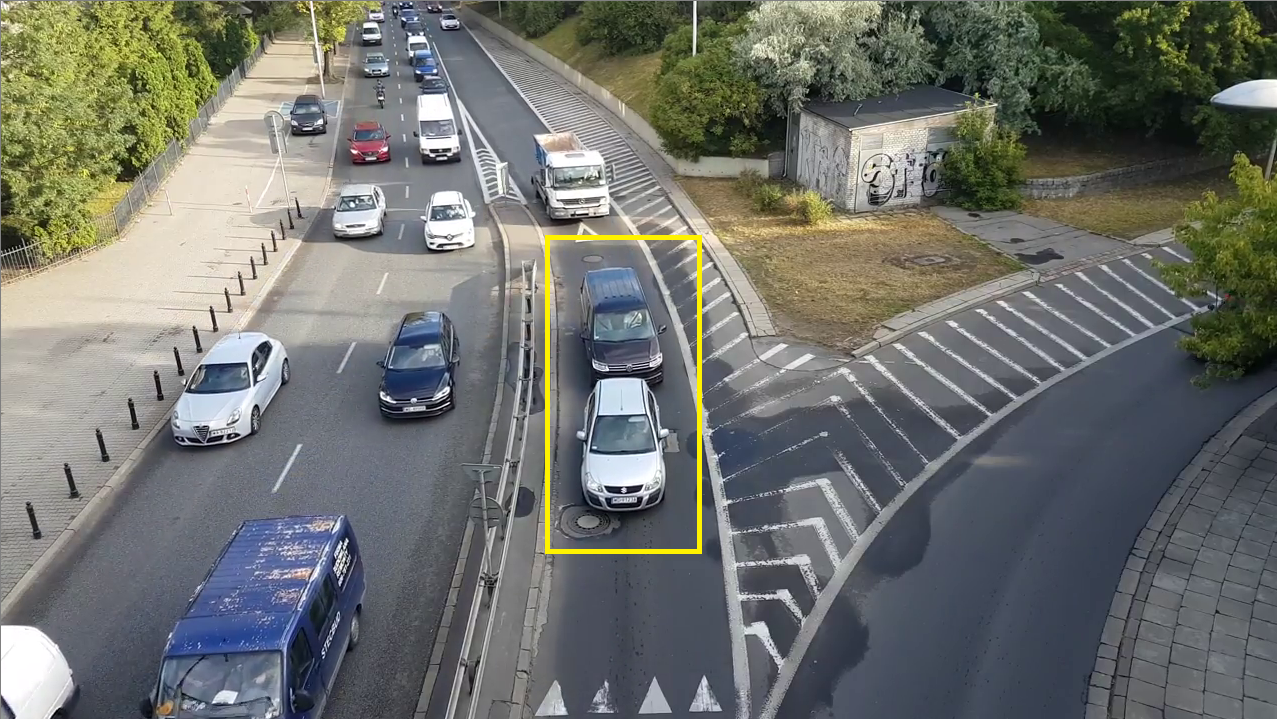
\includegraphics[width = \textwidth]{design/detection/calibration/original}
        \caption{Original Frame - vehicles moving.}
    \end{subfigure}%
    \begin{subfigure}[b]{0.4\linewidth}
        \centering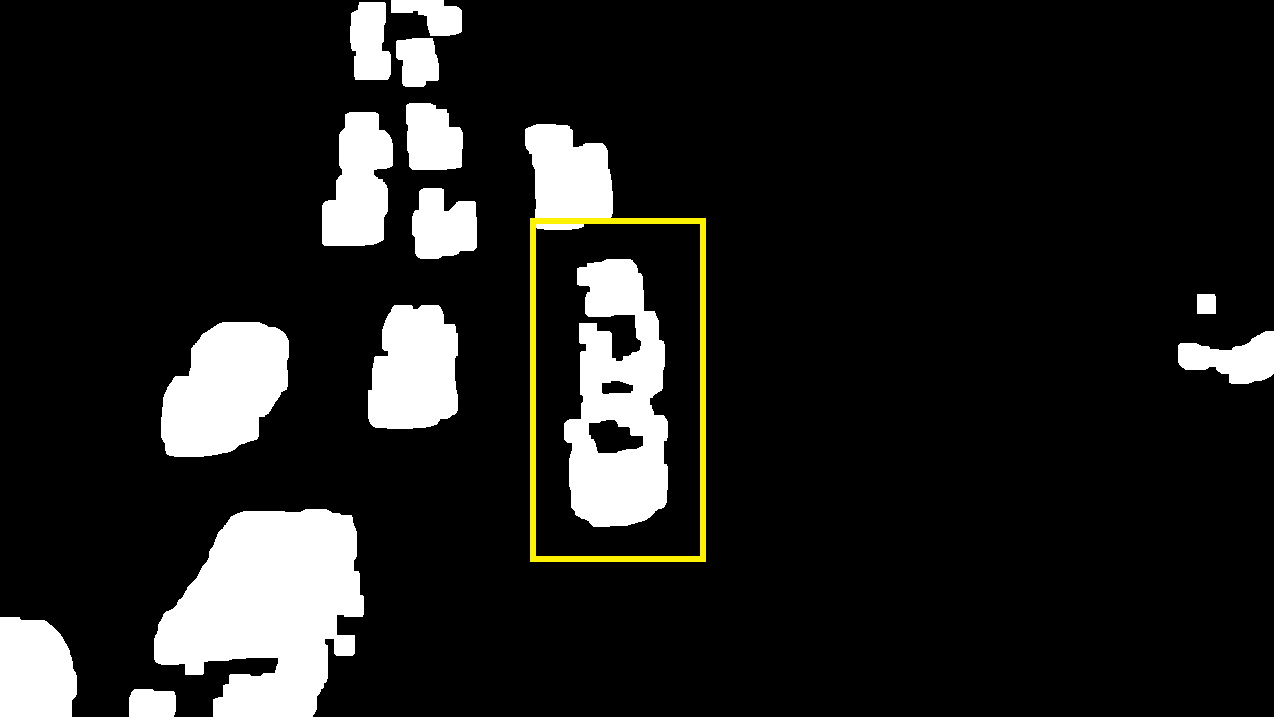
\includegraphics[width = \textwidth]{design/detection/calibration/mask}
        \caption{Foreground Mask - vehicles moving.}
    \end{subfigure}
    \begin{subfigure}[b]{0.4\linewidth}
        \centering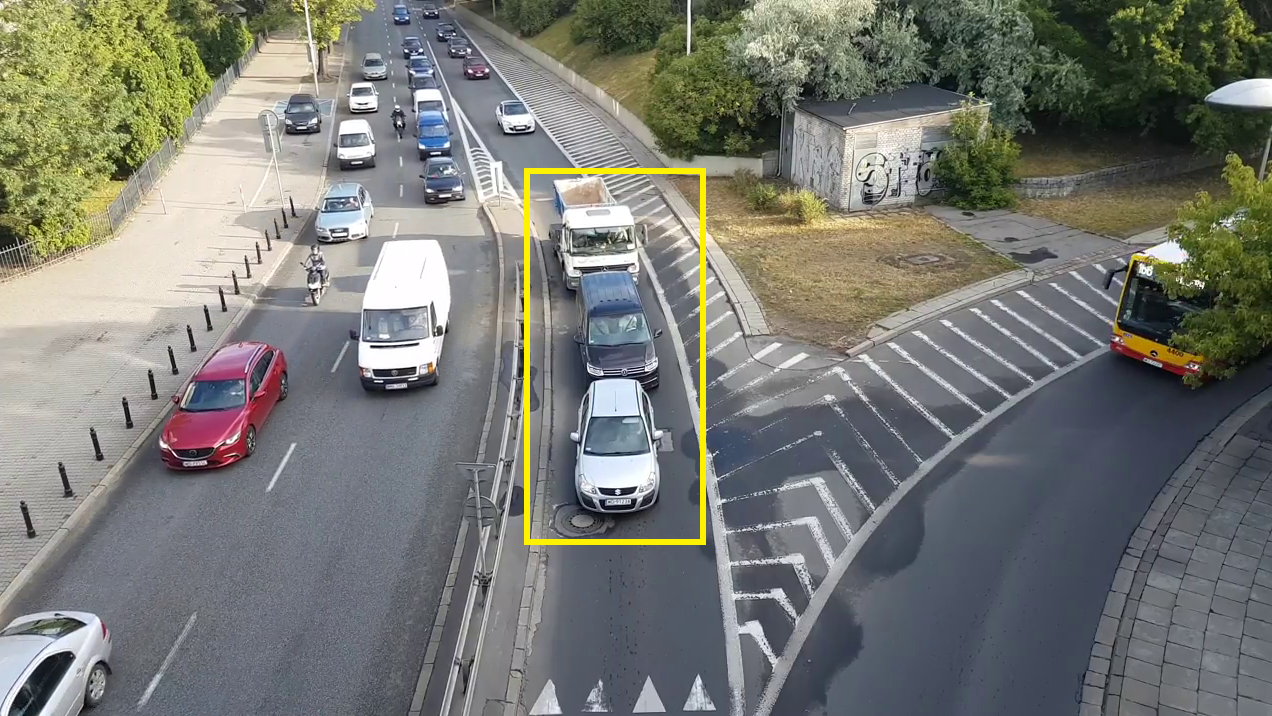
\includegraphics[width = \textwidth]{design/detection/calibration/original_adapted}
        \caption{Original Frame - vehicles stopped.}
    \end{subfigure}%
    	\begin{subfigure}[b]{0.4\linewidth}
        \centering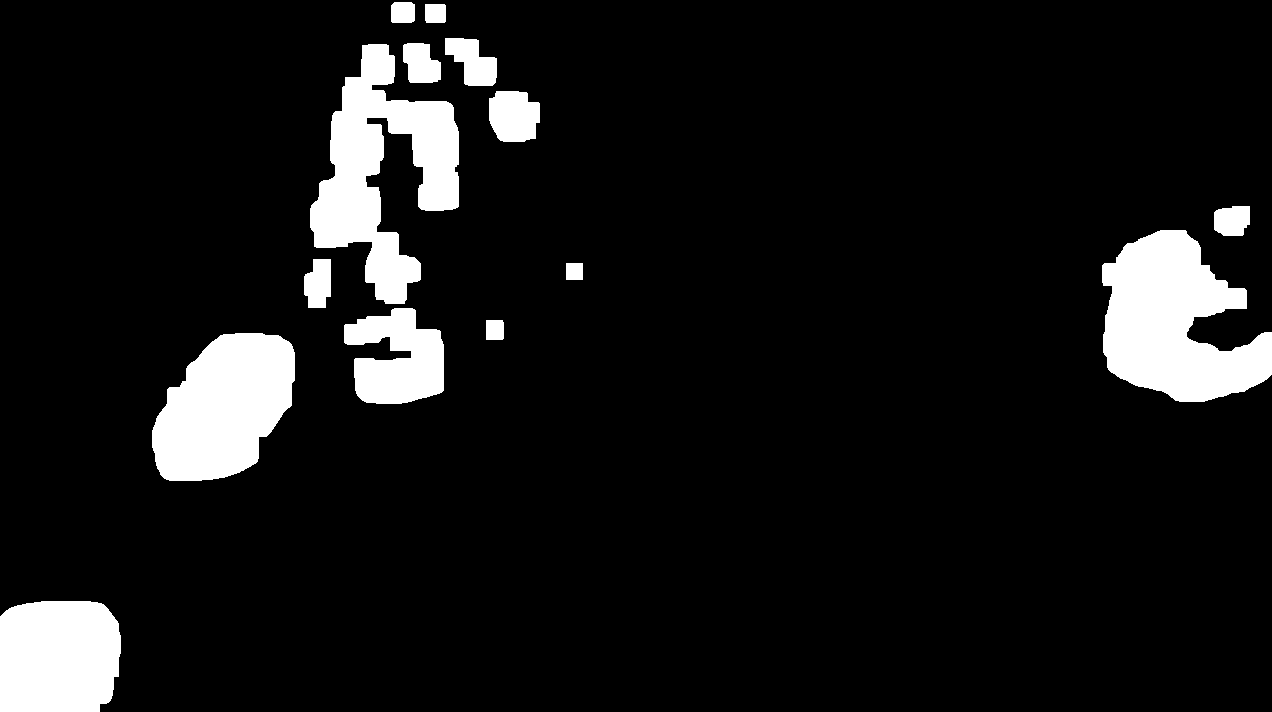
\includegraphics[width = \textwidth]{design/detection/calibration/mask_adapted}
        \caption{Foreground Mask - vehicles stopped.}
    \end{subfigure}
    \caption{Adaptation GMM background cluster. Images by Karol Majek}
    \label{fig:cluster_adaptation}
\end{figure}


